%%%%%%%%%%%%%%%%%%%%%%%%%%%%%%%%%%%%%%%%%%%%%%%%%%%%%%%%%%%%%%%%%%%%%%%%%%%%%%%%%%%%%%%

%   8888888b.                                         888      888
%   888   Y88b                                        888      888
%   888    888                                        888      888
%   888   d88P 888d888 .d88b.   8888b.  88888b.d88b.  88888b.  888  .d88b.
%   8888888P"  888P"  d8P  Y8b     "88b 888 "888 "88b 888 "88b 888 d8P  Y8b
%   888        888    88888888 .d888888 888  888  888 888  888 888 88888888
%   888        888    Y8b.     888  888 888  888  888 888 d88P 888 Y8b.
%   888        888     "Y8888  "Y888888 888  888  888 88888P"  888  "Y8888

%%%%%%%%%%%%%%%%%%%%%%%%%%%%%%%%%%%%%%%%%%%%%%%%%%%%%%%%%%%%%%%%%%%%%%%%%%%%%%%%%%%%%%%

% vscode extension LaTex-Workshop uses these magic comments to 
% define which program will be used to build the project or bibliography
% I do need lualatex to use markdown package. Also, when I use lualatex
% in need to include `pdfencoding=auto` in hyperref setup.
% !TEX program = lualatex

% `-shell-scape` argument doesn't work in Windows 10 lualatex
%% !TEX options = -synctex=1 -interaction=nonstopmode -shell-scape "%DOC%"
% !TEX options = -synctex=1 -interaction=nonstopmode "%DOC%"
% !BIB program = biber

\documentclass[11pt,a4paper,dvipsnames,twoside]{article}

% Document geometry
\usepackage[a4paper,left=3cm,right=2.5cm,vmargin=2.5cm]{geometry}
% \usepackage[showframe,a4paper,left=3cm,right=2.5cm,vmargin=2.5cm]{geometry}

% inputenc is ignored when I'm using lualatex as builder
% \usepackage[utf8]{inputenc}

% To produce a spanish automated output, for instance, TOC is called 'Índice' and
% References is called 'Referencias' (in this case I prefer english)
\usepackage[english]{babel}

% Modifier for space between lines (=\baselinestretch*\baselineskip)
% \renewcommand{\baselinestretch}{1.5}
% Modifies the space between notes in footnotes 
% IMPORTANT: just the same than paragraphs (parskip package below)
% \setlength{\footnotesep}{.9\baselineskip}

% It is better to use setspace package
\usepackage{setspace}
\setstretch{1.5}

% Modifies the space over footnote line
\addtolength{\skip\footins}{\baselineskip}

% To convert fonts already installed in the system and using them as main font in the document
% To check the names that fontspec admits use `otfinfo -i </path/to/font/file/even.ttf>`
% otfinfo does admit also ttf files! For instance:
% `otfinfo -i /usr/share/fonts/liberation/LiberationSerif-Regular.ttf`
\usepackage{fontspec}
\setmainfont{Liberation Serif}
\setsansfont{Liberation Sans}
\setmonofont{CourierPrimeCode-Regular} 
% \setmonofont{Liberation Mono}
% A different font for titles
\newfontfamily\headingfont[]{Liberation Sans}

% To allow custom headings
\usepackage[compact]{titlesec}
\titleformat*{\section}{\Large\headingfont\bfseries}
\titleformat*{\subsection}{\large\headingfont\bfseries}
\titleformat*{\subsubsection}{\normalsize\headingfont\bfseries}
% To control spacing for sections, I'm not using it, it just an example
% \titlespacing*{\section}{3em}{0em}{-2em}

% To change title font family
% \usepackage{titling}
% \renewcommand{\maketitlehooka}{\headingfont}

% To change TOC appearance; see 2.1 section in tocloft.pdf for info about 'titles' option
% it does not mention fancyhdr package but it do the work to flushright page numbers for 
% table of contents pages. see: https://tex.stackexchange.com/a/137301/83189
% \usepackage[titles]{tocloft}
\usepackage{tocloft}
\renewcommand{\cftsecfont}{\headingfont\bfseries}
\renewcommand{\cftsecpagefont}{\headingfont\bfseries}
\renewcommand{\cftsubsecfont}{\headingfont}
\renewcommand{\cftsubsecpagefont}{\headingfont}
\renewcommand{\cftsubsubsecfont}{\headingfont}
\renewcommand{\cftsubsubsecpagefont}{\headingfont}
\tocloftpagestyle{fancy} % However, I find better this way bc 'titles' option does not 
% produce a compact TOC, it does expand bc probably it uses the same spacing rules in 
% the TOC than in (subsub)(sub)sections titles at the rest of the text.
% -------------------
% Remove the TOC title (it is redundant if you have included a TOC section inside TOC)
\makeatletter
\renewcommand{\@cftmaketoctitle}{}
\makeatother
% But in the case you still want to print the TOC title, this other one modifies TOC title font
\renewcommand{\cfttoctitlefont}{\Large\headingfont\bfseries}


%%%%%%%%%%%%%%%%%%%%%%%%%%%%%%%%%%%%%%%%%%%%%%%%%%%%%%%%%%%%%%%%%%%%%%%%%%%%%%%%%%%%%%%

%   8888888b.                   888
%   888   Y88b                  888
%   888    888                  888
%   888   d88P 8888b.   .d8888b 888  888  8888b.   .d88b.   .d88b.  .d8888b
%   8888888P"     "88b d88P"    888 .88P     "88b d88P"88b d8P  Y8b 88K
%   888       .d888888 888      888888K  .d888888 888  888 88888888 "Y8888b.
%   888       888  888 Y88b.    888 "88b 888  888 Y88b 888 Y8b.          X88
%   888       "Y888888  "Y8888P 888  888 "Y888888  "Y88888  "Y8888   88888P'
%                                                      888
%                                                 Y8b d88P
%                                                  "Y88P" 

%%%%%%%%%%%%%%%%%%%%%%%%%%%%%%%%%%%%%%%%%%%%%%%%%%%%%%%%%%%%%%%%%%%%%%%%%%%%%%%%%%%%%%%

% biblatex package
% 'block=nbpar' produces a new paragraph for every block (printing the URLs in a new line and preventing breaking short URLs)
% page 50 in https://osl.ugr.es/CTAN/macros/latex/contrib/biblatex/doc/biblatex.pdf
\usepackage[block=par,style=ieee,backend=biber]{biblatex}
\addbibresource{Paper.bib}
\setcounter{biburllcpenalty}{7000}
\setcounter{biburlucpenalty}{7000}
\setcounter{biburlnumpenalty}{7000}

% Basic packages (they don't need extra configurations)
\usepackage{% `esvect` will not work without texlive-fontsextra
  amsmath,
  amsfonts,
  amssymb,
  graphicx,
  multirow,
  tabularx,
  mathtools,
  color,
  url
}

% Improve captions in figures
\usepackage[margin=2.5cm]{caption}
\usepackage{subcaption}
% \setlength{\textfloatsep}{1\baselineskip plus 2\baselineskip minus 2\baselineskip}
% \setlength{\intextsep}{1\baselineskip plus 2\baselineskip minus 2\baselineskip}
% \setlength{\textfloatsep}{1\baselineskip}
\setlength{\intextsep}{1\baselineskip}


% Extra colors
\usepackage[x11names,table]{xcolor}

% To cross references and metadata
\usepackage[]{hyperref}
\hypersetup{%
  pdfencoding=auto,
  pdftitle={Degree Final Project},
  pdfauthor={Javier Fernández // jfernandil@alumnos.unex.es},
  pdfsubject={},
  pdfkeywords={Project, Dendrometry, LoRa, Arduino, IoT},
  colorlinks = false,
  linkbordercolor = DarkGoldenrod2,
  urlbordercolor= DarkGoldenrod2,
  %linkcolor = black,
  %urlcolor  = black,
  breaklinks
}

% To make the frame around UEx seal
\usepackage{mdframed}

% To include References and TOC in the TOC
\usepackage[]{tocbibind}

% To avoid 'underfull box' warning caused because bibliography line-break
\usepackage{etoolbox}
\apptocmd{\thebibliography}{\raggedright}{}{}

% To use \begin{markdown}\end{markdown} environment and be able to type markdown mode
% IMPORTANT: do not use indent inside \begin{markdown}\end{markdown} environment in the code! 
% if you do lualatex is not translating the markdown code.
\usepackage{markdown}

% To get proper skips between paragraphs when you left a blank line in the code! (so I don't need to use `\\` 
% and I'm not getting warnings all the time) 
% IMPORTANT:
% here is an interesting article speaking about paragraphs an indentation, there are two types of paragraphs; 
% - classic: using indentation to distinguish between one and another
% - modern: dispenses with indents and instead distinguish paragraphs using a blank line between them
% Commenting/uncommenting the following package you can choose between two types.
% more info here: https://tex.stackexchange.com/a/196941/83189
% However this package also has options, which can be
% `indent` (to enable indentation)
% `skip=.5\baselineskip` (by default)
% `parfill` (to impose a minimum space at the end of the last line of a paragraph =30pt by default)
% \usepackage[skip=\baselineskip]{parskip}
% Another different option
% https://tex.stackexchange.com/a/371986/83189
\parskip=.75\baselineskip
\parindent=0pt

% To make quotes (I need renewcommand for mkbegdispquote and mkenddispquote to enable quote marks at the
% end and beginning to displayquote environment. More info: https://tex.stackexchange.com/questions/101809/how-to-force-csquotes-to-show-the-quotations-marks-in-block-quotes)
\usepackage[style=english]{csquotes}
% \renewcommand{\mkbegdispquote}[2]{\openautoquote}
% \renewcommand{\mkenddispquote}[2]{\closeautoquote#1#2}
% \renewcommand{\mkcitation}[1]{ #1}

% Switching to quoting package (for block quotes, I still need csquotes for \enquote{})
\usepackage[begintext=``, endtext='']{quoting}
\quotingsetup{vskip=5pt}

% To print units
\usepackage{siunitx}

% Enumerate lists
\usepackage{enumitem}
% To fix spaces between paragraphs, items and top or bottom fo enumerate/itemize environments I need the following
% see page 3 in https://osl.ugr.es/CTAN/macros/latex/contrib/enumitem/enumitem.pdf
\setlist[itemize]{%
  parsep=.75\baselineskip,
  topsep=0pt,
  partopsep=0pt,
  itemsep=0pt
}
\setlist[enumerate]{%
  parsep=.75\baselineskip,
  topsep=0pt,
  partopsep=0pt,
  itemsep=0pt
}

% To backrefs in the footnotes
\usepackage{footnotebackref}

% To improve headers an footers (I'm using to set page number at right)
\usepackage{fancyhdr}
% Turn on the style
\pagestyle{fancy}
\fancyhf{} % Start with clearing everything in the header and footer
\renewcommand{\headrulewidth}{1pt} % Removes the horizontal rule in header by default
\fancyfoot[R]{\thepage} % Set the right side of the footer to be the page number
\fancyhead[R]{\rightmark}
\setlength{\headheight}{14pt}% ...at least 51.60004pt


% To insert json snippets
\usepackage{listings}
\renewcommand{\lstlistingname}{Example}
% \lstset{%
  % aboveskip=1\baselineskip plus 1\baselineskip minus 2\baselineskip,
  % belowskip=1\baselineskip plus 1\baselineskip minus 2\baselineskip
% }
% \lstset{aboveskip=-18pt plus 2pt, belowskip=-18pt plus 2pt}

% \colorlet{punct}{red!60!black}
% \definecolor{background}{HTML}{EEEEEE}
% \definecolor{delim}{RGB}{20,105,176}
% \colorlet{numb}{magenta!60!black}
\definecolor{punct}{HTML}{0064d3}
\colorlet{background}{gray!20}
\definecolor{delim}{HTML}{ff0000}
\definecolor{numb}{HTML}{0f9d58}

\lstdefinelanguage{json}{%
  % aboveskip=\baselineskip,
  % xleftmargin=2em,
  basicstyle=\scriptsize\ttfamily,
  numbers=left,
  numberstyle=\scriptsize,
  stepnumber=1,
  numbersep=8pt,
  showstringspaces=false,
  breaklines=true,
  frame=lines,
  backgroundcolor=\color{background},
  literate=
   *{0}{{{\color{numb}0}}}{1}
    {1}{{{\color{numb}1}}}{1}
    {2}{{{\color{numb}2}}}{1}
    {3}{{{\color{numb}3}}}{1}
    {4}{{{\color{numb}4}}}{1}
    {5}{{{\color{numb}5}}}{1}
    {6}{{{\color{numb}6}}}{1}
    {7}{{{\color{numb}7}}}{1}
    {8}{{{\color{numb}8}}}{1}
    {9}{{{\color{numb}9}}}{1}
    {:}{{{\color{punct}{:}}}}{1}
    {,}{{{\color{punct}{,}}}}{1}
    {"}{{{\color{punct}{"}}}}{1}
    {\{}{{{\color{delim}{\{}}}}{1}
    {\}}{{{\color{delim}{\}}}}}{1}
    {[}{{{\color{delim}{[}}}}{1}
    {]}{{{\color{delim}{]}}}}{1},
}

\newcommand\YAMLcolonstyle{\color{red}\mdseries}
\newcommand\YAMLkeystyle{\color{black}\mdseries}
\newcommand\YAMLvaluestyle{\color{blue}\mdseries}
% here is a macro expanding to the name of the language
% (handy if you decide to change it further down the road)
\lstdefinelanguage{yaml}{%
  keywords={true,false,null,y,n},
  keywordstyle=\color{darkgray}\bfseries,
  basicstyle=\YAMLkeystyle\scriptsize\ttfamily,
  numbers=left,
  numberstyle=\scriptsize,
  numbersep=8pt,
  breaklines=true,
  frame=lines,
  backgroundcolor=\color{background},
  sensitive=false,
  comment=[l]{\#},
  morecomment=[s]{/*}{*/},
  commentstyle=\color{purple}\ttfamily,
  stringstyle=\YAMLvaluestyle\ttfamily,
  moredelim=[l][\color{orange}]{\&},
  moredelim=[l][\color{magenta}]{*},
  moredelim=**[il][\YAMLcolonstyle{:}\YAMLvaluestyle]{:},   % switch to value style at :
  morestring=[b]',
  morestring=[b]",
  literate = {---}{{\ProcessThreeDashes}}3
             {>}{{\textcolor{red}\textgreater}}1     
             {|}{{\textcolor{red}\textbar}}1 
             {\ -\ }{{\mdseries\ -\ }}3,
}

% To highlight text with automated line break or 'Overfull \hbox' messages
\usepackage{soul}
\soulregister\enquote7

% To add an extra level in sections
\usepackage{titlesec}
\titleclass{\subsubsubsection}{straight}[\subsection]
\newcounter{subsubsubsection}[subsubsection]
\renewcommand\thesubsubsubsection{\thesubsubsection.\arabic{subsubsubsection}}
\renewcommand\theparagraph{\thesubsubsubsection.\arabic{paragraph}} % optional; useful if paragraphs are to be numbered
\titleformat{\subsubsubsection}
  {\normalfont\normalsize\bfseries}{\thesubsubsubsection}{1em}{}
\titlespacing*{\subsubsubsection}
{0pt}{3.25ex plus 1ex minus .2ex}{1.5ex plus .2ex}
\makeatletter
\renewcommand\paragraph{\@startsection{paragraph}{5}{\z@}%
  {3.25ex \@plus1ex \@minus.2ex}%
  {-1em}%
  {\normalfont\normalsize\bfseries}}
\renewcommand\subparagraph{\@startsection{subparagraph}{6}{\parindent}%
  {3.25ex \@plus1ex \@minus .2ex}%
  {-1em}%
  {\normalfont\normalsize\bfseries}}
\def\toclevel@subsubsubsection{4}
\def\toclevel@paragraph{5}
\def\toclevel@paragraph{6}
\def\l@subsubsubsection{\@dottedtocline{4}{7em}{4em}}
\def\l@paragraph{\@dottedtocline{5}{10em}{5em}}
\def\l@subparagraph{\@dottedtocline{6}{14em}{6em}}
\makeatother
\setcounter{secnumdepth}{4}
\setcounter{tocdepth}{4}

% To include random paragraphs with \blindtext
\usepackage{blindtext}

%%%%%%%%%%%%%%%%%%%%%%%%%%%%%%%%%%%%%%%%%%%%%%%%%%%%%%%%%%%%%%%%%%%%%%%%%%%%%%%%%%%%%%%

%    .d8888b.                                                              888
%   d88P  Y88b                                                             888
%   888    888                                                             888
%   888         .d88b.  88888b.d88b.  88888b.d88b.   8888b.  88888b.   .d88888 .d8888b
%   888        d88""88b 888 "888 "88b 888 "888 "88b     "88b 888 "88b d88" 888 88K
%   888    888 888  888 888  888  888 888  888  888 .d888888 888  888 888  888 "Y8888b.
%   Y88b  d88P Y88..88P 888  888  888 888  888  888 888  888 888  888 Y88b 888      X88
%    "Y8888P"   "Y88P"  888  888  888 888  888  888 "Y888888 888  888  "Y88888  88888P'

%%%%%%%%%%%%%%%%%%%%%%%%%%%%%%%%%%%%%%%%%%%%%%%%%%%%%%%%%%%%%%%%%%%%%%%%%%%%%%%%%%%%%%%

% Provides the \doubt{} command
\newcommand{\doubt}[1] {\textbf{\color{Red3}#1}}
% Provides \lang{} command to mark language doubts
\newcommand{\lang}[1] {\textbf{\color{Tomato1}#1}}

% Provides the \cmd{} command; using soul package and previous \letcolor
% definition for listings package. Read page 3 of soul.pdf or 
% https://tex.stackexchange.com/a/231647/83189
% I need that to get a correct and automated line break when the command I want
% to highlight is too long and is placed at the end of the line.
\sethlcolor{background}
\newcommand{\cmd}[1] {\hl{\texttt{#1}}}


%%%%%%%%%%%%%%%%%%%%%%%%%%%%%%%%%%%%%%%%%%%%%%%%%%%%%%%%%%%%%%%%%%%%%%%%%%%%%%%%%%%%%%%

%   88888888888 d8b 888    888
%       888     Y8P 888    888
%       888         888    888
%       888     888 888888 888  .d88b.
%       888     888 888    888 d8P  Y8b
%       888     888 888    888 88888888
%       888     888 Y88b.  888 Y8b.
%       888     888  "Y888 888  "Y8888

%%%%%%%%%%%%%%%%%%%%%%%%%%%%%%%%%%%%%%%%%%%%%%%%%%%%%%%%%%%%%%%%%%%%%%%%%%%%%%%%%%%%%%%

\title{\headingfont%
  University of Extremadura\\
  Faculty of Science\\[1cm]
  \textbf{%
  	Physics degree\\
    Degree Final Project\\[3cm]
    \flushleft{\large{Developement of a FIWARE-based application for tree species monitoring (dendrometry)}}\\[3cm]
    %\flushleft{\large{About implementation of LoRa-based wireless monitoring systems for tree species dendrometry.}}\\[3cm]
  }
}

% I've used that \parbox to flush right the author, but I must have use this package https://osl.ugr.es/CTAN/macros/latex/contrib/titling/titling.pdf
\author{%
  \parbox{.9\textwidth}{
    \begin{flushright}
      Javier Fernández Aparicio\\
      % $\blacktriangledown$\\
      \href{mailto:jfernandil@alumnos.unex.es}{jfernandil@alumnos.unex.es}\\[\dimexpr\baselineskip + 1cm]
      July 2020
    \end{flushright}
  }
}
\date{}


%%%%%%%%%%%%%%%%%%%%%%%%%%%%%%%%%%%%%%%%%%%%%%%%%%%%%%%%%%%%%%%%%%%%%%%%%%%%%%%%%%%%%%%

%   888888b.                     d8b               8888888b.
%   888  "88b                    Y8P               888  "Y88b
%   888  .88P                                      888    888
%   8888888K.   .d88b.   .d88b.  888 88888b.       888    888  .d88b.   .d8888b
%   888  "Y88b d8P  Y8b d88P"88b 888 888 "88b      888    888 d88""88b d88P"
%   888    888 88888888 888  888 888 888  888      888    888 888  888 888
%   888   d88P Y8b.     Y88b 888 888 888  888      888  .d88P Y88..88P Y88b.
%   8888888P"   "Y8888   "Y88888 888 888  888      8888888P"   "Y88P"   "Y8888P
%                            888
%                       Y8b d88P
%                        "Y88P"

%%%%%%%%%%%%%%%%%%%%%%%%%%%%%%%%%%%%%%%%%%%%%%%%%%%%%%%%%%%%%%%%%%%%%%%%%%%%%%%%%%%%%%%

% To manage hyphenation (words break at end of the line), in this case is to prevent "Tellink" breakage.
\hyphenation{Tellink}

\begin{document}
\noindent % to prevent the indentation before first minipage and be able to expand minipages
\begin{minipage}[t]{.28\textwidth}
    \centering
      \begin{mdframed}[innerbottommargin=490pt, innertopmargin=40pt, linewidth=1pt]
        
\includegraphics[width=\textwidth]{../pictures/Seal/marca-uex-2-color.png}
      \end{mdframed}
\end{minipage}
\hskip 30pt minus 5pt % It is a dynamic space (glue) that starts on 30pt and is 5pt shrinkable
\begin{minipage}[t]{.6\textwidth}
  \centering
  \vspace{1cm}
  \maketitle
\end{minipage}
\thispagestyle{empty}
\newpage
\begingroup
  \thispagestyle{empty}
  \null%
\endgroup
\newpage
% \pagenumbering{arabic}% Arabic page numbers (and reset to 1)
\setcounter{page}{1}
\tableofcontents

\newpage

\phantomsection\section*{Abstract}
\addcontentsline{toc}{section}{Abstract}%
This document gives a detailed description of this project, which is focused on researching possibles low-cost alternatives for wireless dendrometry systems. Currently there exist a lot of expensive and professional systems in the market, that's because this project is intended to reduce costs and increase the versatility, scalability and accessibility.

In order to reach these objetives the project will be supported over free software such as FIWARE\cite{Fiware} or free hardware such as Arduino\cite{Arduino} and Raspberry Pi\cite{Raspberrypi}.

\section{Introduction}
This project arises itself from a direct interaction with professionals inside forestal sector. The original idea was to give technical coverage for particular necessities which professionals in this sector had to face off with. At this point is easy to notice this solution will need to be a distributed solution, due high samples dispersion. \lang{As can be seen}, there are even remote techniques to predict this sample density/dispersion using remote methods which predicts \doubt{between $157$-$170$ indviduals per hectare}\cite{ForestStandVol} (depending on the used model). So according to this and sample size determination theories, to get a great resolution could be necessary a big size for samples and the necessity of a big wireless network of distributed devices, since each device will correspond with an individual.

This is more or less, the definition of the IoT (Internet of Things) concept; according to the abstract in \cite{IoTOverview} IoT concept comes from an earlier concept called M2M (Machine-to-Machine) communications. However, also according to \cite[p.~1(71)]{IoTOverview} there is not an official definition for IoT concept, but according to \cite[p.~2(920)]{IoTObjetives}

\begin{quoting}
  based on the traditional information carriers including the Internet, telecommunication  network  and  so  on,  Internet  of Things (IoT) is a network that interconnects ordinary physical  objects  with  the identifiable addresses  so that provides intelligent services.
\end{quoting}

This, at least, covers a little part what this project is intended to do: \enquote{Interconnect ordinary physical objects with the identifiable adresses} to provide intelligent services. These physical objects are in this case ordinary dendrometers.

Over the years there have existed analog and manual dendrometers, thus data acquisition had to follow a manual process in the same way. This could turn out bothering because the big size for this statistical population, \lang{¿as/like? it was exposed ¿before/above?}. So it was traditionally necessary to go there and as part of the field work, take individual by individual the whole sample data.


\subsection{Dendrometry, a formal definition}
The GEMET (General Multilingual Environmental Thesaurus) adopts the definition for \textit{dendrometry} from \cite{DictNaturalRes}:

\begin{quoting}
  The measuring of the diameter of standing trees from the ground with a dendrometer that can also be used to measure tree heights.
\end{quoting}

This one is a bit wide definition because nowadays most dendrometry researches are focused on stem diameter; however, at this point could be interesting to extend this project to include also a sensor to heights measurement.\footnote{This project is already considered extensive enough.} 

A lot of comercial dendrometry systems are available in the market, nevertheless more than single and manual dendrometers those are complex and professional distributed systems, consequently \lang{¿like/as?} has been already said, one of the most important objectives in this project is to research about the possibility to get lower the costs of the whole system, because those professional systems are still expensive. So this is intended to get a cheaper system and make it accessible to everyone who wants \lang{to monitorize} one or more trees growth. 

There are quite a few types of dendrometers but according to \cite{DendroResearch} \enquote{It is possible to define two broad categories of dendrometer: those that contact the stem and those that do not}. This project is focused on the former kind, so for this project is being developed a \enquote{contact dendrometer} based on a linear potentiometer.


\subsection{Hardware}

\subsubsection{Arduino, multipurpose microcontroller}
It's not difficult to justify the use of such an interesting platform as Arduino. The adaptability is one of its strengths, therefore; it is able to acquire and process certain data coming from a set of sensors and manage it to send this via any plugged wireless network interface.

Due circumstances exposed in introduction section is needed an accessible and multipurpose platform \lang{to be the basis for the device design itself}, this is to say the core part of the dendrometer is an Arduino microcontroller.  

Since the idea is to produce a low-cost device in order to distribute a high number of them, it must be a simple design; that's because it consist only of three parts,

\begin{itemize}
  \item \href{https://es.rs-online.com/web/p/products/0317780/}{\doubt{Linear potentiometer:}} which is the sensor itself due is directly in contact with the stem. In order \doubt{to improve data acquisition it will be necessary to use a High Input Impedance Amplifier.}
  \item Arduino microcontroller: this is the core part for the device, it will be responsible for acquire linear potentiometer data and send it to a gateway through LoRa interface. 
  \item LoRa interface: similar to other existing wireless interfaces, it is necessary to forward the sensor data to a concentrator (gateway). Usually and due its complexity these kind of interfaces are integrated circuits which are mounted on a PCB in order to obtain a pluggable card/shield. 
\end{itemize}

% I need to use that \texorpdfstring{}{} for the left-side ToC in PDF viewers, because the ® cannot be rendered in there.
\subsubsection{\texorpdfstring{LoRa\textsuperscript{\textregistered} (Lo{\normalfont\sffamily ng} Ra{\normalfont\sffamily nge})}{LoRa® (Long Range)}}
LoRa is a \enquote{long-range, low-power, low-bitrate, wireless telecommunications system}\cite[]{LoRaGeneral}. This is because some devices inside IoT paradigm tend to be economical and low-resources devices, in order to get them distributed/scattered, as it has been pointed. So this low availability (of resources) along with their tendency to be distributed/scattered causes the necessity for a low-power consumption and a long-range telecommunication.

In a more general sense, there is a wider concept to include all these kind of technologies which fullfil the IoT communication requirements, this is the \enquote{Low-Power Wide Area Networks} (LPWAN), so as claimed by \cite[]{LoRaGeneral}

\begin{quoting}
  Colloquially  speaking,  an LPWAN is supposed to be to the IoT what WiFi was to consumer networking: offering radio coverage over a (very) large area by way of base stations and adapting transmission rates, transmission power, modulation, duty cycles, etc., such that end-devices incur a very low energy consumption due to their being connected.
\end{quoting}

It is important to note that \lang{when talking about \enquote{low-power consumption}, in many cases it is actually meaning} battery-powered devices, for example.

By other hand, LoRa can commonly refer to two distinct layers; a physical layer (LoRa itself) and a MAC layer protocol (LoRaWAN). The former one (the physical layer), is a proprietary technology developed by Semtech. So this does mean this layer is not fully open; LoRaWAN, however, is a protocol built to use LoRa physical layer,  It is intended to sensor networks, wherein those sensors exchange packages with some server with a \enquote{low data rate and relatively long time intervals (one transmission per hour or even days).}\cite[p.~9]{LoRaGeneral}. This particularly means that LoRaWAN protocol is perfect for the purpose of this project.  

In comparison with other common telecommunication technologies, LoRa uses lower bandwidth, but it reaches longer distances:

\begin{figure}[htp]
  \centering
  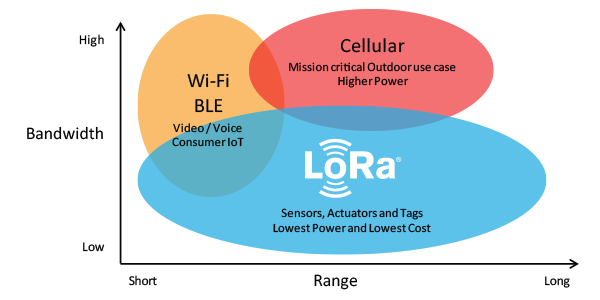
\includegraphics[width=.9\textwidth]{../pictures/LoRa_Why_Range.png}
  \caption{Bandwidth vs range plot for two of the most used telecommunication systems and LoRa.}
  \label{fig:LoraComparison}
\end{figure}
 
\subsubsection{Raspberry Pi, a powerful microcomputer}
As in the case of Arduino, Raspberry Pi provides a powerful platform, however in the case of a Raspberry Pi this platform is slightly more complex than for an Arduino.\footnote{There are a lot of Arduino models, and maybe some of them could be able to support, for example, multiple kind of Real Time Operative Systems, but it is not the case of this project, wherein the Arduino role is just to act as a core for the nodes.} From the hardware point of view, Raspberry Pi implements a better one than Arduino, this also has an impact on a higher cost; however, this hardware allows a Raspberry Pi to support a whole operating system; that's because this devices are usually called \textit{single-board computers}.

A few of interesting hardware specs are for instance, a \textit{Broadcom BCM2837B0, Cortex-A53 (ARMv8) 64-bit SoC @ 1.4GHz} as its CPU, \textit{1GB LPDDR2 SDRAM}, \textit{Gigabit Ethernet over USB 2.0 (maximum throughput 300 Mbps)} or even an \textit{Extended 40-pin GPIO header} among others.\cite{RPiSpecs}

The role for Raspberry Pi in this project is to act like a gateway, receiving all the data from different nodes. So in order to perform this task correctly it is necessary to provide a LoRa interface, which is also embebed (as in Arduino) in a separate pluggable shield/card/hat.

\subsubsection{Dragino shields/hats}\label{sssec:DraginoShields}
These shields/expansion cards are necessary because those devices (Arduino and Raspberry Pi) have not the ability to comunicate through LoRa physical layer, that's because they need a physical interface in order to manage those LoRa packages. Both shields are based on the SX1276/SX1278 transceiver. However the Raspberry Pi hat also has a L80 GPS interface (Base on MTK MT3339), meanwhile Arduino has not.

This project is using the following models: 

\begin{itemize}
  \item \textit{LoRa GPS HAT for Raspberry Pi,}\cite{DraginoRpiHat} which makes use of the extended 40-pin GPIO header to be plugged\footnote{It is important to note this LoRa HAT is not actually designed to play a gateway role, in fact, this is considered a \enquote{Hack where a node-class radio tries to impersonate a gateway}\cite{RpiHatHack},\doubt{(I'm not sure about this citation (It's a forum))} so this means this hat is designed to be a node-class radio, not a gateway.}
  \item \textit{LoRa Shield for Arduino}\cite{DraginoArdShield}, which is plugged through analog and digital pins.
\end{itemize}

\subsection{Software}

\subsubsection{FIWARE}
It is defined as \enquote{The Open Source Platform for Our Smart Digital Future}\cite{Fiware}; in a deeper sense is \enquote{an open source initiative defending an universal set of standards for context data management}\cite{Fiware}, which basically means that \textit{FIWARE} is an open source platform where develop IoT and smart solutions. The platform provides a number of software modules called \textit{Generic Enablers}; among all those \textit{Generic Enablers} there is one particularly important called \textit{Orion Context Broker}. In fact, for a solution to be considered as \textit{Powered by FIWARE} it must to use the \textit{Orion Context Broker} at least. 

This \textit{Context data} is just a way to name any kind of data coming from any kind of sensor. \textit{Orion Context Broker} is designed to manage this context data through concepts such as \textit{subscriptions} or \textit{entities}, to name but a few; however, all these \textit{Generics Enablers} communicate with each other using the \textit{FIWARE NGSI RESTful API}\cite{NGSI}.\footnote{\textit{RESTful} term comes from the software architectural style \textit{REST}, which stands for \textit{Representational State Transfer}}

% \newpage
% \section{Background}
\newpage
\section{Technical description}
Like in the Introduction, the most proper way to present this technical description is to difference between software and hardware parts. However, is still interesting to present a simple and general diagram for whole designed solution:

\begin{figure}[htp]
  \centering
  
\includegraphics[width=.73\textwidth]{../schemes/main_scheme_tbg.png}
  \caption{General view of this solution.}
  \label{fig:GenView}
\end{figure}

\subsection{Hardware}

\subsubsection{Nodes}
Nodes are the parts of the system in direct contact with trees themselves (one node per each tree). Most important features in those devices are: low-cost, low-powered, wireless communication and small size. The following diagram shows a diagram of its most relevant parts:

\begin{figure}[htp]
  \centering
  
\includegraphics[width=.9\textwidth]{../schemes/node_tbg.png}
  \caption{Diagram for a detailed view of a node.}
  \label{fig:NodeDiag}
\end{figure}

This diagram shows three different parts: 

\begin{itemize}
  \item A linear potentiometer, ideally an \href{https://docs.rs-online.com/37bf/0900766b814f0bd0.pdf}{RS Pro Conductive Polymer
  Potentiometer for Automotive Applications}, however, by circumstances is not possible to use it and in order to perform a kind of proof of concept, \doubt{this project will implement a regular rotary potentiometer.}
  \item \doubt{A signal conditioning stage, which is needed in order to improve the quality of the voltage signal produced by the potentiometer.}
  \item Arduino + Dragino LoRa Shield; of course it is necessary to schedule data transmission and acquisition, as well as transmit them using the LoRa physical layer and LoRaWAN protocol. For this purpose an Arduino-like microcontroller is perfect.  
\end{itemize}

\subsubsubsection{Linear Potentiometer}
As said, ideally this potentiometer should be a linear potentiometer with $5\ \si{\kilo\ohm}$ of maximum resistance, however, in order to improve its performance, it's recommended to use it as a voltage divider; also it would be convenient to buffer the resulting output with a high impedance amplifier, that's because the figure \ref{fig:NodeDiag} includes a signal conditioning stage, which will be described below.

\subsubsubsection{Signal conditioning}
This stage is focused on improve the signal acquisition, according to this potentiometer specifications, the best way to achieve this objetive is using a high input amplifier, in fact, a single-supply, rail-to-rail operational amplifier is the best option. \doubt{Here is shown a possible schematics for this stage:}

\begin{figure}[htp]
  \centering
    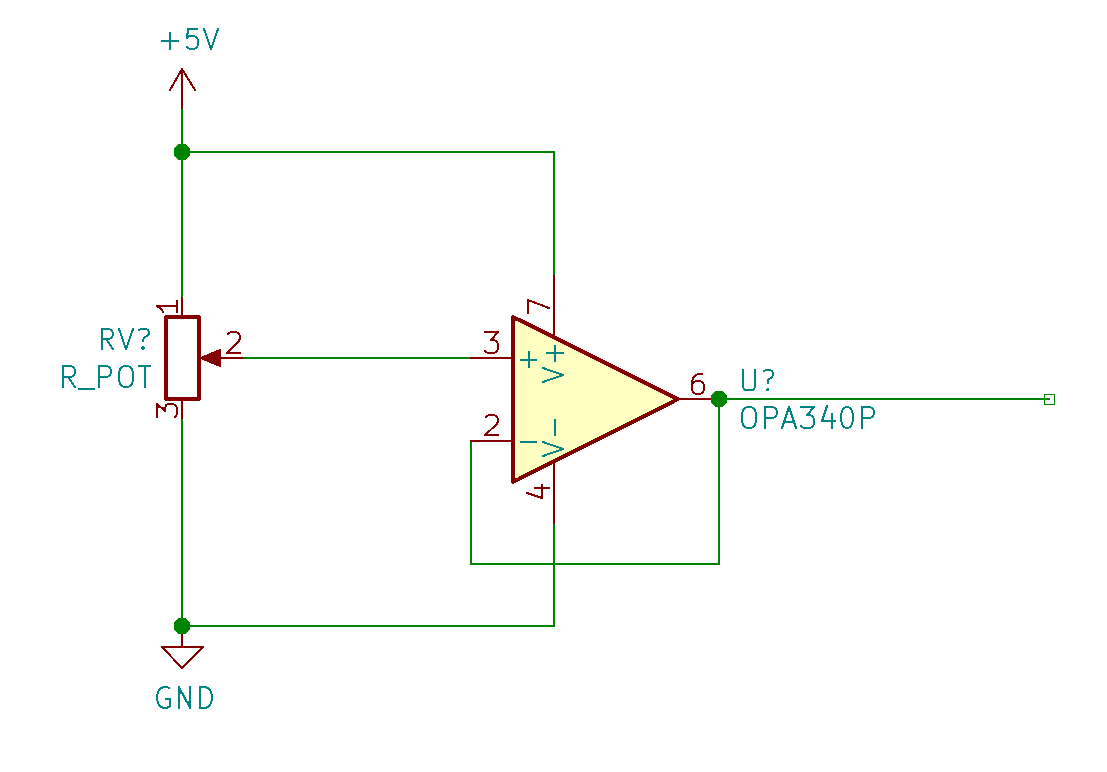
\includegraphics[width=.9\textwidth]{../schemes/Signal_Conditioning.png}
  \caption{Signal conditioning stage.}
  \label{fig:SignalCond}
\end{figure}



\subsubsection{Gateway}

\subsubsubsection{Raspberry Pi 3 B+}
This model of Raspberry Pi is able to run almost every GNU/Linux distribution ported to ARM architecture, Raspberry Pi OS, formerly known as Raspbian,\cite{RaspberryPiOs} is in fact a Debian port to ARM architecture. After a little researching, it is possible to conclude that there is not other operative system which improves the performance of Raspberry Pi OS in a Raspberry Pi. Due this former argument this project is going to use Raspberry Pi OS. 

One of the most interesting features of Raspberry Pi is precisely that OS is installed and run from a microSD card, so the hardware is loading the operative system from this microSD card to the RAM directly, which improves notably the system load times, and increments its portability.

Raspberry Pi foundation provides the \href{https://www.raspberrypi.org/downloads/noobs/}{\textit{Raspberry Pi Imager}} to perform the installation in a microSD card.\footnote{There are many ways to perform the Raspberry Pi OS installation in a microSD card, this document leaves it to readers to use their preferred method. However, this document also considers the \textit{Raspberry Pi Imager} method as the best one.} This tool allows the reader to choose between three different versions of Raspberry Pi OS. Recommended, Lite and Full version. Lite version is the same than Recommended version but without graphical user interface (GUI or Desktop Environment), meanwhile Full version is the same than Recommended version but with a few extra applications. 

This project is using the Recommended version for Raspberry Pi OS, nevertheless, the project does not require absolutely the desktop environment, so to maximize the available free space in the SD card, is better to install the Lite version instead of the Recommended version. 

\begin{figure}[htp]
  \centering
  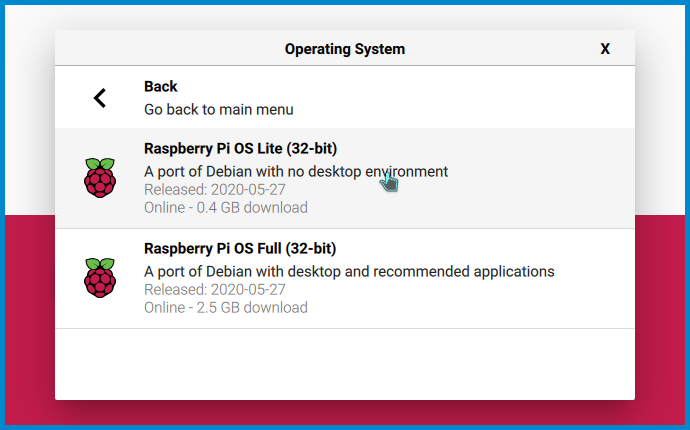
\includegraphics[width=.7\textwidth]{../pictures/rpi_imager.png}
  \caption{Raspberry Pi Imager showing different options to install Raspberry Pi OS in a microSD card.}
  \label{fig:RpiImager}
\end{figure}

Even so, independently of the installed version, the reader will be able to disable the graphical environment using the console based \cmd{raspi-config} application \cite{RaspiConf}. 

One of the first and most important configurations is the internet access; this can be done via two different ways, using the ethernet port (which does not require any extra configuration, just tu plug the cable) or using the WiFi interface, which can be configured using also \cmd{raspi-config} \cite{RaspiWIFIcli}. Due to its versatility, there are multiple setup that could fulfil the requirements of this projects:

\begin{itemize}
  \item \textbf{PoE} (Power-over-Ethernet); this is not actually a suitable option because Raspberry Pi does not support PoE by itself, it needs a \href{https://www.raspberrypi.org/products/poe-hat/}{separate HAT} which is using the GPIO connector, so this makes impossible to use it along the LoRa HAT. Apparently there are hacks to reduce this HAT size, but they also use pins in the GPIO connector \cite{RaspiPoEHack}. Besides, this method only works with up to 100m cables, so it would be necessary to have a power source and internet access point within a 100m radius.\footnote{The \href{https://github.com/hallard/LoRasPI}{LoRasPI HAT} is more suitable for this option because does not cover whole GPIO connector, leaving free the GPIO pins used in \cite{RaspiPoEHack}.}
  \item \textbf{WiFi} and battery powered; this setup implies also the existence of a relatively close power source, because the access point used to provide that wireless network connection should work also with mains power. Probably the WiFi radio is not enough to make it the difference between this setup and the next one suggested.
  \item Simple \textbf{ethernet} and mains power, this setup is similar to the previous one exposed, but omitting the WiFi limitations/configurations, the access point and the Raspberry Pi should be practically both at the same location.
  \item \textbf{GSM module} and battery or mains powered; this document consider this the ideal setup. This setup doesn't require a conventional access point because the internet access is granted through a GSM module, in a similar way than a mobile phone. This would be the ideal way because it minimizes the resources needed, which is crucial in an environment where those probably won't be available ---in the middle of the forest.
  
  Furthermore, this is apparently possible through two different options:
    \begin{itemize}
      \item \href{https://www.itead.cc/wiki/RPI_SIM800_GSM/GPRS_ADD-ON_V2.0}{Itead Raspberry Pi GSM Board (SIM800)}. This is not the most interesting way, because though GPIO pins comes through this does mean the HAT supports \href{http://www.pi-in-the-sky.com/index.php?id=stacking-guide}{stacking}, and even if that does, doesn't mean every other HAT would.
      \item \href{https://tutorials-raspberrypi.com/raspberry-pi-gsm-module-mobile-internet-lte-3g-umts/}{USB GSM module}. This is apparently the most promising option. These kind of GSM modules are in general compliant with GNU/Linux systems and using a regular SIM card, they would be eventually able to provide an internet access point. Of course, this also will to increment the size of the whole device.
    \end{itemize}
\end{itemize}

It is important to note the necessity of a relatively stable internet connection; those gateways will forward the traffic to the cloud server, so they are receiving LoRa packets through its LoRa interface and then forwarding them to the specified server. 

Another configuration which must be done is the Secure Shell (\cmd{ssh}) service; which according to Raspberry Pi documentation can be done from terminal using \cmd{systemd} \cite{RaspiSSH}. 

So generating a pair of keys and configuring properly the ssh access; it will probably be necessary to paste the \cmd{*.pub} key content into \cmd{~/.ssh/authorized\_keys} file (located in the local folder in the Raspberry Pi); and give it the right permissions (\cmd{700}), after this the reader should be able to connect through ssh service.

\begin{lstlisting}[%
    % float=ht,
    language=json,
    firstnumber=1,
    caption={Creating a pair of ssh keys.},
    label=ej:CreateEntity
    ]
    $ ssh-keygen
    Generating public/private rsa key pair.
    Enter file in which to save the key (/home/wyre/.ssh/id_rsa): 
    Enter passphrase (empty for no passphrase): 
    Enter same passphrase again: 
    Your identification has been saved in /home/wyre/.ssh/id_rsa
    Your public key has been saved in /home/wyre/.ssh/id_rsa.pub
    The key fingerprint is:
    SHA256:vkNRk/Fo8iGGo0pYlwb2L3vf3TgOfm11MmZW+BipXgQ wyre@DESKTOP-AFG84JJ
    The key's randomart image is:
    +---[RSA 3072]----+
    |  o       .o     |
    | . o . .  +oE    |
    |  . = o +.+... o |
    | o o o o.= .  = .|
    |. . o . S..  o = |
    | . . o ..   . O +|
    |  . . ... .. * +.|
    |     . ..+ o+oo  |
    |        o.oo+o.  |
    +----[SHA256]-----+
\end{lstlisting}

Once is available the remote control for Raspberry Pi through ssh, is possible to manage it completely from the command line, even upgrade the system and compile the required controller to get properly working the LoRa transceiver. 

At this point and depending on the type of access point used to provide internet service to the Raspberry, the reader will be able even to remote control the Raspberry over internet. For this purpose could be useful to read the access point documentation in order to perform port forwarding or alternatively \href{http://www.thirdway.ch/En/projects/raspberry_pi_3g/index.php}{a reverse tunnel over ssh} ---in the case the ISP does not allow ssh when using a GSM module, also the reader may find that IPv6 works but IPv4 does not. Anyway, as said the internet access point could be variable and it is not determined by this project.\footnote{The most important thing is to work comfortably with the Raspberry Pi with no HDMI, keyboard and mouse plugged, and this can be done locally in a LAN to configure it in a first place.}  

\subsubsubsection{Dragino GPS and LoRa HAT}
Gateways doesn't need actually a diagram or detailed description because there are multiple devices which could play this role. These usually are generic devices due LoRaWAN protocol versatility. LoRaWAN is a cloud-based medium access control (MAC) layer protocol, but actually acts as a network layer protocol for managing communication between gateways and nodes, similar to a routing protocol. So it is possible for any device which implements hardware for a LoRa physical layer, to act as a gateway.

Nevertheless, there are important considerations about the said above, for example, nodes are not actually associated with an specific gateway. Instead, data transmitted by a node is typically received by multiple gateways. Each gateway will forward the received packets from the end-node to de cloud-based network server. Besides, this project is using a Raspberry Pi 3B+ with a Dragino Hat which mounts a SX1276 LoRa \textbf{transceiver}\cite{SX1276}; this is so important because means, according to Semtech, this transceiver is not intended to play a gateway role, but a end-node role.

A transceiver, by definition, is a device that is able to both, transmit and receive (in fact, the word itself is a mix between both, \textbf{trans}miter and re\textbf{ceiver}) that is what a node must be able to do; i.e. transmit the sensor data (context) and receive data to perform operations with its actuators. 

Nevertheless, LoRaWAN specification varies from region to region \enquote{based on
the different regional spectrum allocations and regulatory requirements}\cite[p.~12]{LoRaWANspec}. In fact, for Europe, and again as reported by \cite[p.~13]{LoRaWANspec} 

\begin{quoting}
LoRaWAN defines ten channels, eight of which are multi data rate from 250bps to
5.5 kbps, a single high data rate LoRa channel at 11kbps, and a single FSK channel
at 50kbps.
\end{quoting}

Here is the important point. This Dragino HAT for the Raspberry Pi, mounts an SX1276 transceiver, which is known as node-class transceiver, so in conclusion, \textbf{this Dragino LoRa GPS HAT is not LoRaWAN compliant}. The main reason the SX1276 transceiver is not suitable to work as a gateway is that \doubt{it is actually a single channel transceiver}. Despite all of this, there still exist the possibility of use it as a gateway, because it is technically possible. 


Dragino foresees this and provides a dual channel controller \cite{Dragino_DualChannelController_Rpi}. The most important thing about this dual channel controller, is not the possibility to use the transceiver in a dual channel mode, but to use it as a gateway in the physical sense.

In order to get the HAT operative, the reader will need to enable the SPI (Serial Peripheral Interface). This can be done also with \cmd{raspi-config} 

\begin{figure}[ht]
  \centering
  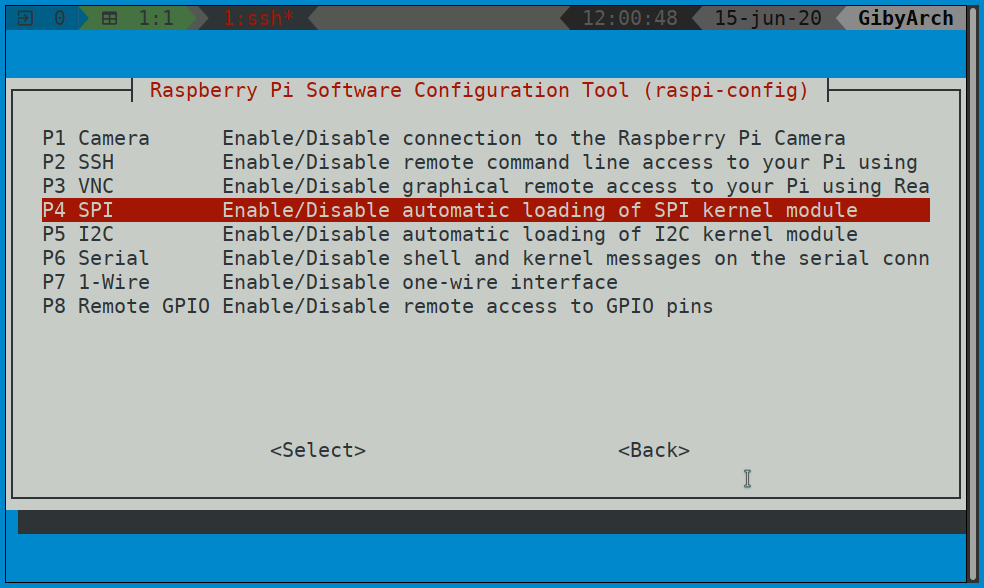
\includegraphics[width=.9\textwidth]{../pictures/SPI_raspi-config.png}
  \caption{SSH session to enable the SPI kernel module in Raspberry Pi using \cmd{raspi-config}. Inside \enquote{5 Interfacing options}}
  \label{fig:EnablingSPI}
\end{figure}

Then it would be necessary to install the GPIO access library from Raspberry repositories, \cmd{sudo apt install wiringpi}. After this, the reader will be in position to clone the controller from the github repository \cite{Dragino_DualChannelController_Rpi}

\begin{lstlisting}[%
  % float=ht,
  language=json,
  firstnumber=1,
  caption={Instructions to compile and install as a system service},
  label=ej:compiling_dual_channel_pkg
  ]
  cd ~
  git clone https://github.com/dragino/dual_chan_pkt_fwd
  cd dual_chan_pkt_fwd
  make
\end{lstlisting}

Once the controller is compiled, the reader must check the contents of \cmd{global\_conf.json}, for this projects, due it is using the LoRa GPS HAT Single Channel LoRa \cite{DraginoRpiHat}, the pins configuration in \cmd{global\_conf.json} must be the following as stated by \cite{Dragino_DualChannelController_Rpi}

\begin{lstlisting}[%
  % float=ht,
  language=json,
  firstnumber=1,
  caption={defined pins in \cmd{global\_config.json}},
  label=ej:global_configJSON
  ]
  "pin_nss": 6,
  "pin_dio0": 7,
  "pin_rst": 0
\end{lstlisting}

I order to obtain the gateway ID the reader will need to perform the following command to run for the first time the \cmd{dual\_chan\_pkt\_fwd} binary, i.e. once the compilation process has produced the \cmd{dual\_chan\_pkt\_fwd} binary is necessary to run it directly to check the terminal output and find for the gateway ID.

\begin{lstlisting}[%
  % float=ht,
  language=json,
  firstnumber=1,
  caption={Running for the first time the LoRa HAT controller.},
  label=ej:Running_DualChann_Controller
  ]
  $ sudo ./dual_chan_pkt_fwd
  server: .address = router.eu.staging.thethings.network; .port = 1700; .enable = 1
  server: .address = router.eu.thethings.network; .port = 1700; .enable = 0
  Gateway Configuration
    your name (a@b.c)
    Dual channel pkt forwarder
    Latitude=0.00000000
    Longitude=0.00000000
    Altitude=10
    Interface: eth0
  Trying to detect module CE0 with NSS=6 DIO0=7 Reset=3 Led1=unused
  SX1276 detected on CE0, starting.
  Trying to detect module CE1 with NSS=6 DIO0=7 Reset=3 Led1=unused
  SX1276 detected on CE1, starting.
  Gateway ID: b8:27:eb:ff:ff:1b:14:9b
  Listening at SF7 on 868.100000 Mhz.
  Listening at SF7 on 868.100000 Mhz.
  -----------------------------------
  stat update: 2020-06-15 10:53:04 GMT no packet received yet 
\end{lstlisting}

After this last instruction (\cmd{sudo make install}) the 




\subsection{Software}






















\phantomsection
\addcontentsline{toc}{section}{References}
\printbibliography
\end{document}
